\documentclass[a4paper]{IEEEtran}

\usepackage{xcolor}
\usepackage{hyperref}
\usepackage[utf8]{inputenc}
\usepackage[pdftex]{graphicx} 
\usepackage{multirow, pgfplotstable,booktabs,colortbl,lmodern}

\newcommand\TODO{\textcolor{red}{[TODO]}}
\newcommand\todo[1]{\textcolor{red}{[TODO: #1]}}
\newcommand\CN{\textcolor{blue}{[Citation Needed]}}
\newcommand\cn[1]{\textcolor{blue}{[Citation Needed: #1]}}

\title{The Cellular Automata Research Platform: PCIe}
\author{Per Thomas Lundal}

\begin{document}

\maketitle

\begin{abstract}

\TODO

\end{abstract}

\section{Introduction}

Something about von Neumann's seminal work on self-replication from around 1950 \cite{neumann1966theory}.
Insight into origins of life.


\section{Related Work}

Evolution
\begin{itemize}
    \item Genetic Algorithm
\end{itemize}

Artificial Development (Harding, Banzhaf)
\begin{itemize}
    \item Zygote
    \item Scalability
    \item Robustness
    \item Plasticity
\end{itemize}

\section{Previous Work}

\ref{fig:ca-djupdal}
\ref{fig:ca-aamodt}
\ref{fig:ca-stovneng}

\begin{figure}[h!]
    \centering
    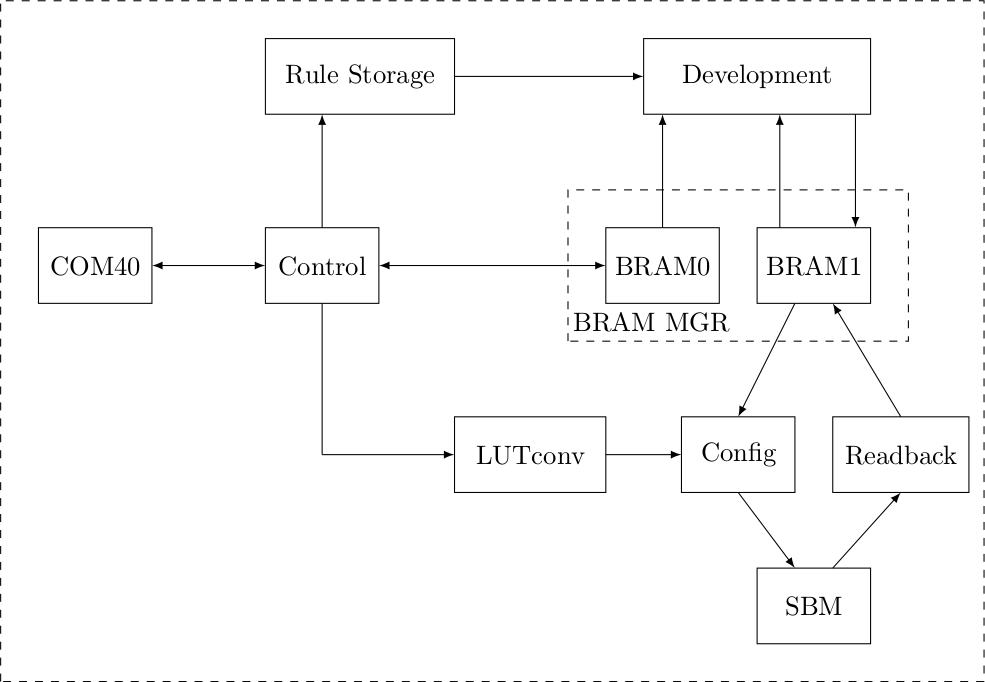
\includegraphics[width=0.5\textwidth]{figures/ca-djupdal}
    \caption{Original design by Djupdal}
    \label{fig:ca-djupdal}
\end{figure}

\begin{figure}[h!]
    \centering
    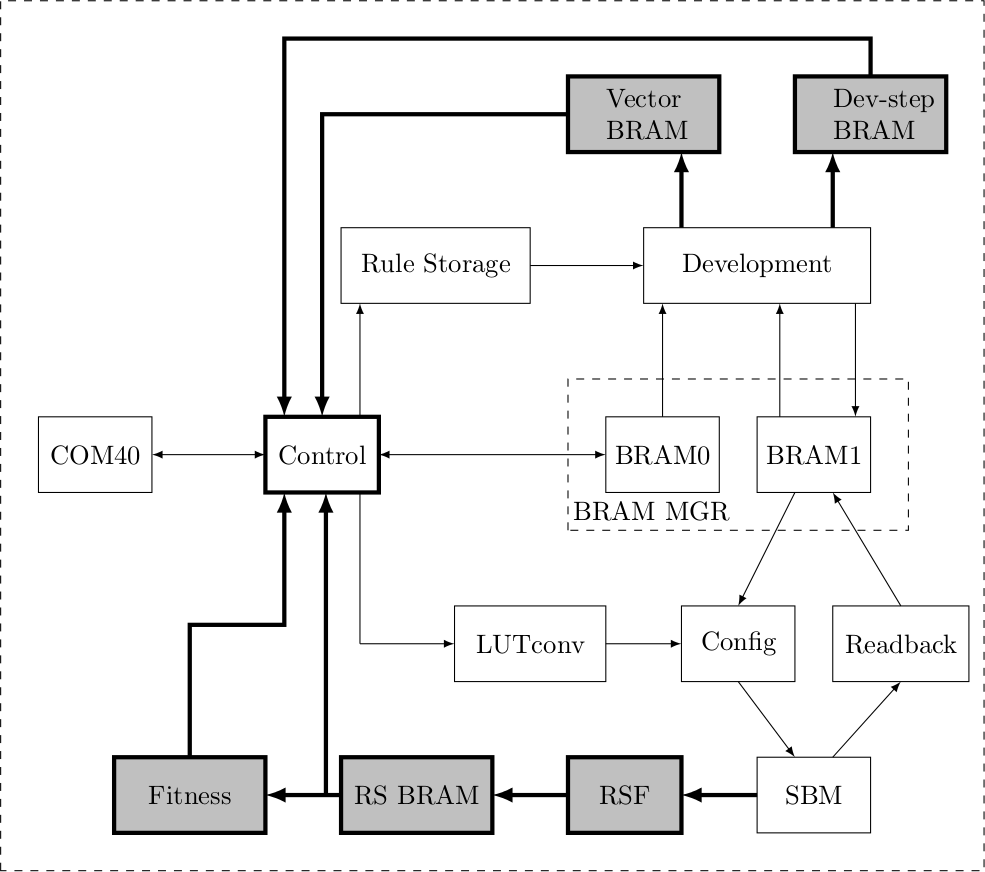
\includegraphics[width=0.5\textwidth]{figures/ca-aamodt}
    \caption{Additions by Aamodt}
    \label{fig:ca-aamodt}
\end{figure}

\begin{figure}[h!]
    \centering
    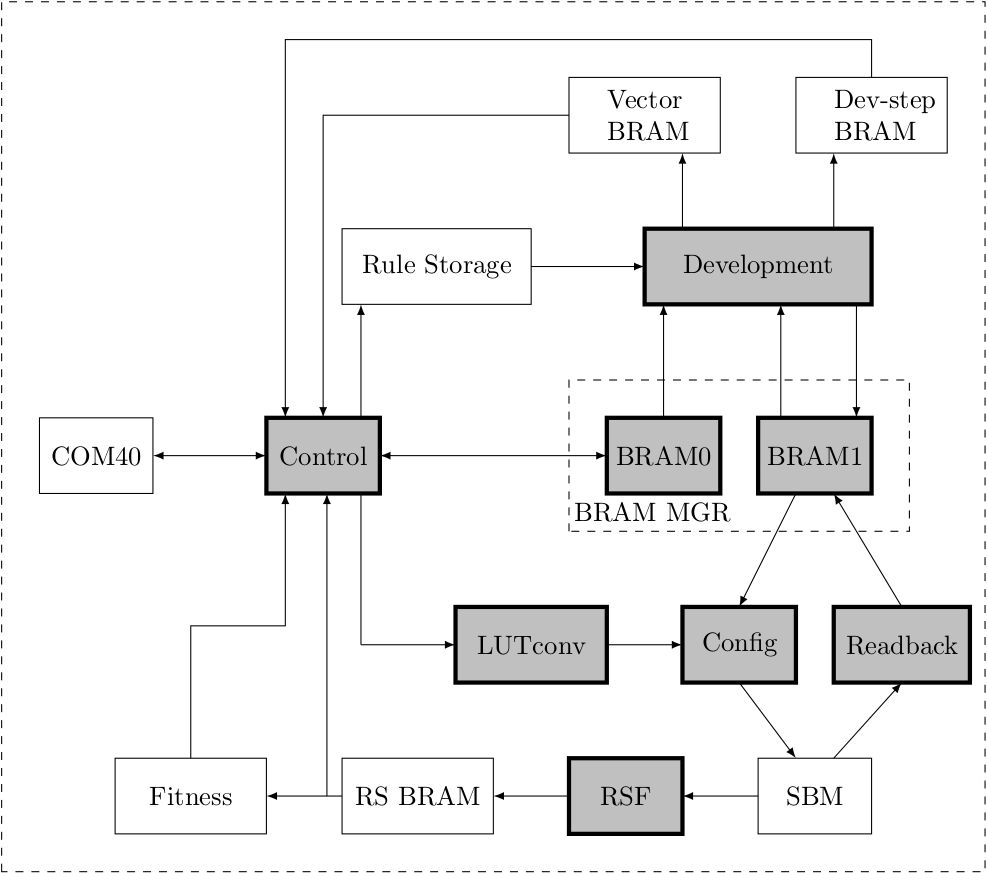
\includegraphics[width=0.5\textwidth]{figures/ca-stovneng}
    \caption{Parts optimized by Stovneng}
    \label{fig:ca-stovneng}
\end{figure}

\section{Methodology}

\TODO

\section{Results}

\TODO

\section{Discussion}

\TODO

\section{Conclusion}

\TODO

\bibliography{bibliography}
\bibliographystyle{plain}
\nocite{*}

\end{document}
